%
% Motivation / Introduction
%
\section{Introduction}
    % <A brief overview of your project suitable for a non-specialised
    % audience. You may mention background and motivation, but should avoid
    % technical terms as far as possible. 1-2 paragraphs should be sufficient.
    % Here is an example of how to cite a reference \cite{parikh1980adaptive}.>

    Current filesystems broadly group into two types: those aimed for everyday
    use, like ext4, and large enterprise-ready solutions like zfs.
    Unfortunately, small home server use, for people who do not wish to use
    cloud or paid storage services, doesn't quite fit either of these two. The
    usual workaround is to use everyday filesystems on top of RAID. However,
    RAID relies on disks to not fail silently. Despite all drives' best effort
    in error correcting, they still occasionally silently corrupt data
    \cite{google_flash, facebook_flash}.

    The usual way to solve this is to add further layers of complexity that
    add some sort of checksumming on top of RAID, like Backblaze
    \cite{backblaze} or Google \cite{google_fs} do. The home server tools act
    in a similar manners (eg Linux's dm-integrity).

    The idea for this project is to produce a filesystem and then integrate
    these features - redundancy and integrity - to use out of the box with
    little configuration. It should, in a sense, be a drop-in replacement for
    the everyday filesystem for simpler administration.

%
% Aims, Objectives and deliverables.
%
\section{Aims, Objectives and Delievarables}

\subsection{Project Aims}
    % <A brief summary of the primary aims of this project. Typically 1-3
    % sentences.>

    This project aims to produce a new redundant filesystem for Linux. It is
    intended to be a more light-weight alternative to the enterprise-ready ZFS
    but to cut down some of its features and only keep those necessary for home
    server use. It should require a lot less system resources and be as
    convenient as an everyday filesystem to use.

\subsection{Objectives}
    % note this means `learn how to\ldots', `research into\ldots` are {\em not}
    % objectives, as they are intermediate milestones rather than final goals.
    % All objectives should be measurable, {\em i.e.} it should be possible to
    % provide evidence to confirm whether or not they have been achieved. 3-5
    % objectives is typical.>

    \begin{description}
        \item[A modern filesystem design]

            The first and most important objective is creating a modern
            filesystem. Modern in the sense that it should be have comparable
            speed to other widespread filesystems, like ext4 and NTFS, and
            provide the most important features users have come to expect.

            Currently, this is expected to include standard inodes organised in
            some B-tree structure of blocks on disk. Blocks will be overwriting
            (instead of copy on write) and will only consider SSDs.

            A major goal is to not depend on an fsck utility. Crashes should be
            automatically detected and corrected on mount.

        \item[A filesystem implementation]

            The design will be implemented as a userfs module for Linux. It
            should be mountable as any other and seamlessly usable.

        \item[Redundancy and silent error correction]

            Since the filesystem will assume flash-based underlying media,
            which is prone to quite a few silent errors despite all the error
            correction features \cite{facebook_flash, google_flash}, the
            filesystem design will make according considerations about speed
            and reliability. It will integrate the redundancy features of RAID
            and provide assurances against data corruption, like block/file
            checksumming, which plain RAID does not. Silent error detection and
            recovery is the main focus for this filesystem.

            The end result should resemble ZFS in spirit, but without all of
            the enterprise considerations. That means fewer system resource
            requirements, less rigorous protection against crashes and higher
            device flexibility, if possible.

        \item[Comparison and evaluation]

            It is expected that the proposed filesystem will offer some
            benefits (at lest for home use) without taking steps back on
            usability and performance. To verify this, extensive testing will
            have to be conducted and the result compared against current
            solutions.

            The goal is the evaluation to drive the design to an extent so that
            the end result does not regress on expected features.

        \item[Illustrative report]

            Although this objective is optional, it is high on the wish list.
            Most filesystems research papers and documentation articles fail to
            illustrate the layout of what they are proposing, instead relying
            on convoluted textual descriptions. The goal is for the final
            report to include some of these graphical descriptions to aid with
            arguments.

    \end{description}


\subsection{Deliverables}
    % <A list of what you will hand in at the end of the project. This will
    % include the final report (possibly spread across multiple deliverables,
    % if that makes sense for your project), code (possibly more than one
    % version), and so on. Ideally the deliverables should be cross-referenced
    % to the objectives. 2-3 deliverables is typical, but there can be more
    % depending on the nature of the project.>

    There are only 2 deliverables: the final report and source code. The report
    will contain all background research, feature considerations, the basis for
    the major proposals and performance analyses. It will have the complete
    design and all evaluations and comparisons. I expect this to include lots
    of graphs and drawings to illustrate tradeoffs. The source code will be a
    working userfs module which can be compiled and loaded into a modern Linux
    operating system to immediately use the filesystem along with the data used
    to perform the analyses.

%
% Plan
%
\section{Project Plan}
    % submission of the final report. This should discuss the key stages of
    % your project.>

    As of writing this report, most preliminary research has been completed.
    Next, are \ref{l1_num} major stages:


    % TODO: Don't do everything from scratch, unless you want to look at it, bc
    % it affects planning
    \begin{enumerate}

        \item Look into B-trees and the layout of ext4/NTFS to get a feel for
            what current filesystems look like. This is not intended to be an
            in-depth look, but rather a guide on how to proceed. Only modern
            examples will be considered.

        \item Immediately after that, research and implement the userfs module.
            This will include a basic layout on disk with a good ordering
            arrangement. Wherever possible, external libraries will be used
            (eg. GQDM for a B-tree implementation). Any housekeeping should be
            taken care of at this stage (mounting/unmounting procedures, system
            calls, etc) and files should be readable and writeable to a disk. A
            development environment should emerge in the process. The current
            idea is that this be done with loopback devices on my development
            machine.

        \item At this stage testing should be considered, especially failure
            simulation. Since the major topic of the project deals with
            handling various failures, which are rather unpredictable
            \cite{google_flash}, there should be some mechanism available to
            insert them reliably. It is likely that this will require the
            development environment be in a virtual machine (QEMU) which will
            be done at this stage if necessary.

            At this point a working, but very barebones prototype should be
            ready. From here until the end of the project the prototype should
            have a consistently working state which should go on until time
            runs out.

        \item Next is where the bulk of the work is expected to happen. There
            are only two mandatory parts to implement: redundancy - replication
            at some granularity like RAID - and reliability - checksumming like
            ZFS'. If time allows, more features will be added to make the
            comparison to existing filesystems more accurate. At the end of
            various increments some testing criteria will be devised to assess
            the viability of the features and make changes accordingly. This is
            expected to be done with already existing benchmarks (eg. fio -
            flexible IO tester) for simplicity, although some academic metrics
            will also be considered, for example the way LFS was benchmarked
            \cite{LFS}.

        \item Finally, although the intention is to write up results for the
            report throughout the project, the bulk of it will happen at the
            end so some judgement will be exercised to cease work, even if
            incomplete, and draw up results for the final report.

            This is when most graph and figures are expected to be drawn so
            that the report is easy to follow.

    \label{l1_num}
    \end{enumerate}


\subsection{Timeline}
    % <A graphical description of your plan, often as a Gantt chart.>

    % To include a figure, uncomment and modify the following. Vary the 'width'
    % field until it looks suitable. This uses the 'graphicx' module that has
    % already been included in 'config.tex'.

    % TODO: make the figure more clear. Implm should be longer?
    \begin{figure}[htbp]
    	\centerline{
    		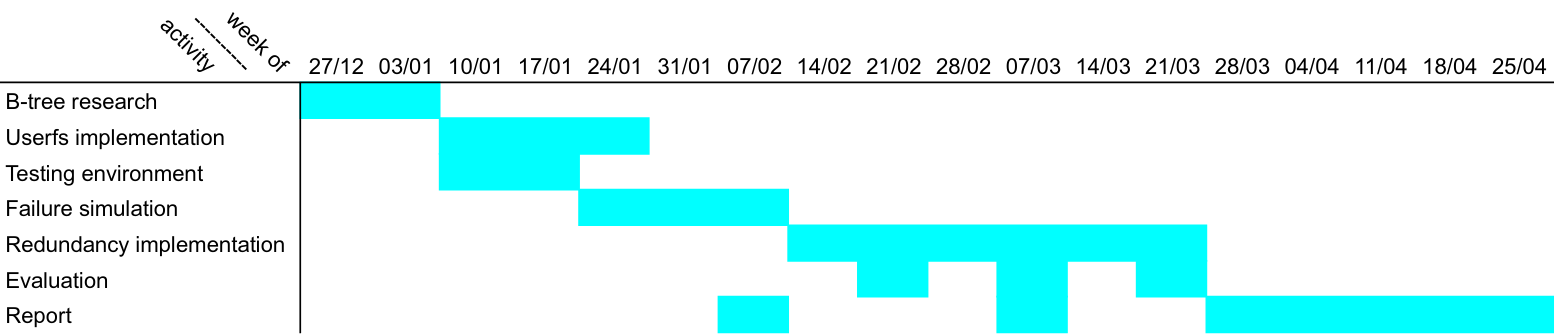
\includegraphics[width=18cm]{gantt}
    	}
    	\caption{Gantt chart of the plan}
    \end{figure}

%
% Risk mitigation.
%
\section{Risk Mitigation}
    % <Identify risks to your project, and what you would do if they arose.>

    This project has a number of risks. It is quite involved and requires a lot
    of new skills. Despite that, it is believed that it is achievable with some
    alterations to the ideal vision for it:

    \begin{description}

        \item[Complex implementation] The biggest risk to this project is
            running out of time due to overwhelming code complexity from
            writing a filesystem driver. Kernel programming is a very elaborate
            exercise and due to a lack of sufficient experience in it, the
            implementation will be done in userspace as a userfs module. This
            certainly diminishes the efficiency of the implementation and may
            skew some performance measurements. However, userspace programming
            experience is plentiful and only has a small fraction of the things
            that could go (inexplicably) wrong. As the focus on of the project
            is not meant as an engineering feat so this should free up time for
            the more important academic aspect of it.

        \item[Incomplete prototype] Despite the reduction in complexity with a
            userfs, a large chunk of the work on the project is not towards
            making a better filesystem, but rather making a filesystem at all.
            To make sure the code is not completely unusable in case some
            feature fails, the project will use a sort of "rolling release"
            model. The idea is to implement and test features individually and
            in whole before starting a new one. If one cannot be implemented
            for whatever reason, the project can be submitted regardless.
            Anything after the initial barebones filesystem should be
            submittable so that even if the project ends up as a glorified
            literature review it can get as many marks as possible.

        \item[Full originality] This project will not attempt to create an
            original and filesystem with novel features. Due to the size and
            complexity of creating a filesystem this is not feasible for a
            final year project. Instead, since there are no originality marks,
            the novelty of the project is going to be very limited. None of the
            features are novel themselves, but the way they are arranged is not
            particularly widespread. This should drastically reduce the chance
            for unforseen problems and get the project off the ground faster.

        \item[Too many devices] Hard drives will not be considered. The whole
            filesystem will be implemented with the expectation that it will
            run on an SSD. This limit the pool of devices that have to be
            considered for any performance impacts.

        % TODO: research: consider only most modern FSs and ignore everything
            % before. Whatever i've learnt, that's it.

    \end{description}

%
% Ethics.
%
\section{Ethics}
    % <If your project has ethical issues (e.g. gathering of user consent
    % forms), then you should state here how you intend to address them. If
    % there are no ethical issues then explicitly state: "There are no ethical
    % issues for this project.">

    This project has no ethical issues. It does not deal with humans in any way
    and only aims to better a set of tools which are widely accepted and
    available.
